\tit{Partial lexicographic preference trees}, or \tit{PLP-trees}, 
is an intuitive formalism that allows compact representation
of qualitative preferences over combinatorial domains.
In this work, we review different classifications of PLP-trees,
and introduce \tit{partial lexicographic preference forests},
or \tit{PLP-forests}, to reduce the high variance of PLP-trees.
To support experimentation, we have constructed a preference
learning library from existing reservoir of classification
datasets.
To this end, we implemented an \tit{exact} learner using
\tit{answer-set programming}, and an \tit{approximation}
learner using a straightforward greedy heuristic.
Our empirical results on PLP-trees show that the language offers
high accuracy, mostly higher than decision trees when training samples
are small.
For PLP-forests, we have observed improvements, significant in some cases,
from single tree models.


\section{Introduction}
Preferences are everywhere and have been extensively studied
by researchers and scientists in artificial intelligence,
psychology, operations research, and social choice theory.

%In the recent decade, the interest on preference learning
%has grown evidently in the literature.
%Learning conditional preference networks (CP-nets)\cite{boutilier2004cp}
%have received tremendous attention.
%However, reasoning tasks for CP-nets are mostly
%computationally hard, e.g., deciding if an outcome
%is preferred to another
%is in general PSPACE-complete\cite{goldsmith2008computational}.

Learning to predict preferences has been an important task across many
areas in computer science.
In label ranking, the task is to learn a model that
maps a given outcome to a preference ranking of the labels.
In classification, the problem is to apprximate
a function by learning a hypothesis that maps an instance
to a classifier; in the preference learning setting,
the instance would be two outcomes, and the classifier could
tell the preference between the two.
Besides this machine learning perspective,
researchers have studied preference learning with
assumptions of the representations of the model to
be learned.
Representations of intuitive meaning and compact size
are especially of interest.
Conditional preference networks (CP-nets)\cite{boutilier2004cp}
is such a formalism, and learning CP-nets have 
received tremendous attention.

Continuing this line of research on representation-based
preference learning,
AI researchers have also proposed and studied preference languages 
exploiting the idea of ordering
outcomes lexicographically,
such as lexicographic strategies\cite{schmitt2006complexity},
conditional lexicographic trees\cite{brauning2012learning},
lexicographic preference trees\cite{booth:learningLP}, and
partial lexicographic preference trees (PLP-trees)\cite{conf/aaai15/LiuT}.

In this work, we focus on the representations of PLP-trees and forests of PLP-trees.
We consider four classes of PLP-trees and their corresponding forests:
\tit{unconditional importance and unconditional preference} (UIUP), 
\tit{unconditional importance and conditional preference} (UICP), 
\tit{conditional importance and unconditional preference} (CIUP), and
\tit{conditional importance and conditional preference} (CICP).
We are given a dataset of pairwise preferences, called \tit{examples}.
First, for each class, we want to learn a PLP-tree that is in agreement
with as many examples in the \tit{training} set as possible,
and test it using the \tit{testing} set to see how well
the model generalizes to the testing data.
Second, for each class, we want to learn a set of PLP-trees, or a forest,
hoping for better performance than a single tree.
To support our experiments,
inspired by the work by Br{\"a}uning and Eyke\cite{brauning2012learning},
we have built a preference learning library of semi-real-world
datasets from classification repositories.

The model of decision trees
in machine learning is different from PLP-trees.
A decision tree classifies whether an outcome is better than another,
but its size usually grows as the training examples, and it does not
directly answer optimal queries.
Some classes of PLP-trees (e.g., UIUP) have size linear
in the size of the attribute domains.
Computing an optimal outcome given a PLP-tree
takes polynomial time in the size of these domains.
Moreover, PLP-trees are arguably more intuitive and 
more cognitively plausible than decision trees.

%This requires translation of the examples in $\cE$ to
%labeled instances.
%For instance, an example $\alpha \succ \beta$ is transformed
%to
%\begin{center}
%	($\alpha$,$\beta$,1) or ($\beta$,$\alpha$,0).
%\end{center}

We outline the rest of the paper as follows.
We will review PLP-trees and its classifications in Section 2,
and introduce and define PLP-forests in Section 3.
Next, in Section 4, we will discuss the datasets in the 
preference learning library built by us, including where the original 
datasets were from, and how we constructed
preferencial datasets for our own use.
In Section 5, we will present and analyze experimental
results obtained by us for learning both
PLP-trees and PLP-forests.
Finally, we will conclude with a brief summary of our work
and a look into possible directions of future work.


\section{Partial Lexicographic Preference Trees}
\nop{\tc{DISCUSS BINARY OR MULTI-VALUED ATTRIBUTES AS OUR EXPERIMENTS ARE ON
BOTH BINARY AND MULTI-VALUED?}}
PLP-trees was originally defined with respect to 
binary attributes\cite{conf/aaai15/LiuT}.
In this work, we expand it to the general case
where attributes are multi-valued.
Let $\cA=\{X_1,\ldots,X_p\}$ be a set of attributes, with each
$X_i$ having its finite domain $D_i$, the size of which is
bounded by a constant.
The corresponding \tit{combinatorial domain} over $\cA$ is the Cartesian product 
$\CD(\cA)=D_1 \times \ldots \times D_p$.
Elements in $\CD(\cA)$ are called \tit{outcomes}.

A PLP-tree over $\CD(\cA)$ is a labeled tree, where every
non-leaf node is labeled by an attribute from $\cA$ and by a preference
entry (a total order over $D_i$), where every leaf node is denoted by a box 
$\Box$, and where non-leaf node has as many outgoing edges,
ordered from left to right according to the preference entry, as there are
values in the domain of the attribute labeling it. 
Moreover, we require that on every path from the root to a leaf
each attribute appears \tit{at most} once. 

To specify the total preorder on outcomes defined by a PLP-tree $T$, let 
us enumerate leaves of $T$ from left to right, assigning them 
integers $1,2$, etc. For every outcome $\alpha$, we find its leaf 
in $T$ by starting at the root of $T$ and proceeding downward. 
When at a node labeled with an attribute $X$, we descend to
some child of that node based on the value $\alpha(X)$ of the attribute $X$ 
in $\alpha$ and on the preference entry assigned to that node. 
If $\alpha(X)$ is the $i$-th preferred value, we descend to the $i$-th child. 
The integer assigned to the leaf that we eventually get 
to is the \tit{rank} 
of $\alpha$ in $T$, written $r_T(\alpha)$. The preorder $\succeq_T$ on 
distinct outcomes determined by $T$ is defined as follows: $\alpha\succeq_T \beta$ 
if $r_T(\alpha)\leq r_T(\beta)$ (smaller ranks are ``better''). We also 
define derived relations $\succ_T$ (strict order) and $\approx_T$ 
(equivalence or indifference): $\alpha \succ_T\beta$ if $\alpha\succeq_T
\beta$ and $\beta \not\succeq_T \alpha$, and $\alpha_T\approx_T\beta$ if 
$\alpha\succeq_T\beta$ and $\beta\succeq_T \alpha$. Clearly, $\succeq_T$ 
is a total preorder on outcomes partitioning them into strictly ordered 
clusters of equivalent outcomes. 
%To simplify the notation, we always drop
%the sbscript $T$  whenever it is clear from the context.

To illustrate the notions just introduced, we consider preference orderings 
of cars over six multi-valued attributes. 
The \tit{BodyType} ($X_1$) can be \tit{minivan} ($x_{11}$), 
\tit{sedan} ($x_{12}$), or \tit{sport} ($x_{13}$).
The \tit{Capacity} ($X_2$) can be \tit{2} ($x_{21}$),
\tit{5} ($x_{22}$), or \tit{7-or-more} ($x_{23}$).
The \tit{Color} ($X_3$) can be \tit{black} ($x_{31}$) or \tit{white} ($X_{32}$). 
The \tit{Make} ($X_4$) is either \tit{Honda} ($x_{41}$) or \tit{Ford} ($x_{42}$).
The \tit{Price} ($X_5$) can be \tit{high} ($x_{51}$), \tit{low}
($X_{52}$), or \tit{medium} ($X_{53}$). 
Finally, \tit{Transmission} ($X_6$) can be \tit{automatic} ($x_{61}$)
or \tit{manual} ($x_{62}$).
An agent could specify her preferences over dinners as a PLP-tree $T$ in 
\figref{PLPT_full_ex}. The \tit{BodyType} is the most important attribute to 
the agent and she prefers minivan, followed by sedan and sport. 
Her next most important attribute is contingent upon what type of cars
the agent is considering.
For minivans, her most important attribute is \tit{Make}, for which
she likes Honda more than Ford.
Among sedans, her most important attribute is \tit{Price}, on which
she prefers medium over low, and low over high.
Amongst sport cars, her top priority is \tit{transmission} and she
prefers manual to automatic.
\begin{figure}[!ht]
	\centering
	\begin{tikzpicture}[->,>=stealth',
	  level 1/.style={sibling distance=2.5cm, level distance=35pt},
		level 2/.style={sibling distance=0.7cm, level distance=30pt},
		level 3/.style={sibling distance=0.4cm, level distance=30pt}]
	  \node [main node,inner sep=1.5pt,label={[xshift=1.2cm, yshift=-0.5cm]$\scriptstyle x_{11}>x_{12}>x_{13}$}] {$X_1$}
	    child {node [main node,inner sep=1.5pt,label={[xshift=-0.9cm, yshift=-0.5cm]$\scriptstyle x_{41}>x_{42}$}] {$X_4$}
	  		child {node [rectangle,draw] {}}
	  		child {node [rectangle,draw,fill] {} edge from parent node[right] {\small{$l_1$}}}
			}
	    child {node [main node,inner sep=1.5pt,label={[xshift=1.2cm, yshift=-0.5cm]$\scriptstyle x_{53}>x_{52}>x_{51}$}] {$X_5$}
	  		child {node [rectangle,draw,fill] {} edge from parent node[left] {\small{$l_2$}}}
	  		child {node [rectangle,draw] {}}
	  		child {node [rectangle,draw] {}}
	    }
	    child {node [main node,inner sep=1.5pt,label={[xshift=0.9cm, yshift=-0.5cm]$\scriptstyle x_{62}>x_{61}$}] {$X_6$}
	  		child {node [rectangle,draw] {}}
	  		child {node [rectangle,draw] {}}
	    };
	\end{tikzpicture}
  \caption{PLP-tree $T$ over the car domain\label{fig:PLPT_full_ex}}
\end{figure}

Let us consider two cars. 
Car $c_1$ is a white Ford minivan with a capacity of 7 or more, 
a middle-range price, and an automatic transmission; that is,
$c_1=\la x_{11},x_{23}, x_{32}, x_{42}, x_{53}, x_{61} \ra$.
Car $c_2$ is a black Honda sedan with a capacity of 2, a middle-range
price, and a manual transmission:
$c_2=\la x_{12},x_{21}, x_{31}, x_{41}, x_{53}, x_{62} \ra$.
Traversing the tree $T$, we see that $c_1$ reaches leaf $l_1$ of rank $2$
and $c_2$ leaf $l_2$ of rank $3$.
We have $r_T(c_1)<r_T(c_2)$. Thus, we see $c_1 \succ_T c_2$.

\begin{figure}[!ht]
	\centering
  \begin{subfigure}[b]{0.5\textwidth}
		\centering
	  \begin{tikzpicture}[->,>=stealth',
	    level 1/.style={sibling distance=2.7cm, level distance=35pt},
			level 2/.style={sibling distance=1.7cm, level distance=35pt},
			level 3/.style={sibling distance=0.7cm, level distance=35pt}]
	    \node [main node,inner sep=1.5pt,label={[xshift=1.2cm, yshift=-0.5cm]$\scriptstyle x_{12}>x_{13}>x_{11}$}] {$X_1$}
	      child {node [main node,inner sep=1.5pt,label={[xshift=-0.8cm, yshift=-0.5cm]$\scriptstyle x_{42}>x_{41}$}] {$X_4$}
	    		child {node [main node,inner sep=1.5pt] {$X_6$}
	  				child {node [rectangle,draw] {}}
	  				child {node [rectangle,draw] {}}
					}
	    		child {node [main node,inner sep=1.5pt,label={[xshift=-0.85cm, yshift=-0.5cm]$\scriptstyle x_{61}>x_{62}$}] {$X_6$}
	  				child {node [rectangle,draw] {}}
	  				child {node [rectangle,draw] {}}
					}
				}
	      child {node [main node,inner sep=1.5pt,label={[xshift=0.9cm, yshift=-0.5cm]$\scriptstyle x_{42}>x_{41}$}] {$X_4$}
	    		child {node [main node,inner sep=1.5pt] {$X_6$}
	  				child {node [rectangle,draw] {}}
	  				child {node [rectangle,draw] {}}
					}
	    		child {node [main node,inner sep=1.5pt,label={[xshift=-0.85cm, yshift=-0.5cm]$\scriptstyle x_{62}>x_{61}$}] {$X_6$}
	  				child {node [rectangle,draw] {}}
	  				child {node [rectangle,draw] {}}
					}
	      }
	      child {node [main node,inner sep=1.5pt,label={[xshift=0.9cm, yshift=-0.5cm]$\scriptstyle x_{42}>x_{41}$}] {$X_4$}
	    		child {node [main node,inner sep=1.5pt] {$X_6$}
	  				child {node [rectangle,draw] {}}
	  				child {node [rectangle,draw] {}}
					}
	    		child {node [main node,inner sep=1.5pt,label={[xshift=-0.85cm, yshift=-0.5cm]$\scriptstyle x_{61}>x_{62}$}] {$X_6$}
	  				child {node [rectangle,draw] {}}
	  				child {node [rectangle,draw] {}}
					}
	      };
	  \end{tikzpicture}
		\caption{Collapsible PLP-tree \label{fig:UICP_PLPT_full}}
	\end{subfigure}\\
  \begin{subfigure}[b]{0.5\textwidth}
		\centering
	  \begin{tikzpicture}[->,>=stealth',
	    level/.style={sibling distance=2.5cm/#1, level distance=35pt}]
	    \node [main node,inner sep=1.5pt] {$X_1$}
	      child {node [main node,inner sep=1.5pt] {$X_4$}
	      	child {node [main node,inner sep=1.5pt] {$X_6$} {}
							child {node [rectangle,draw] at (2.47,3.7) {$x_{12}>x_{13}>x_{11}$} edge from parent[draw=none]}
							child {node [rectangle,draw] at (1.2,2.5) {$x_{42}>x_{41}$} edge from parent[draw=none]}
							child {node [rectangle split, rectangle split parts=3,draw] at (0.75,1.1) 
								{$x_{12}:x_{61}>x_{62}$ \nodepart{second} 
								 $x_{13}:x_{62}>x_{61}$ \nodepart{third}
								 $x_{11}:x_{61}>x_{62}$} edge from parent[draw=none]}
					}
	      };
	  \end{tikzpicture}
		\caption{UICP PLP-tree \label{fig:UICP_PLPT_compact}}
	\end{subfigure}
  \caption{PLP-trees over the car domain}
  \label{fig:UICP}
\end{figure}


\vspace{-0.1cm}
\subsection{Classification of PLP-Trees}

\vspace{-0.1cm}
In the worst case, the size of a PLP-tree is exponential in the number of 
attributes in $\cA$. However, some PLP-trees have a special structure that
allows us to ``collapse'' them and obtain more compact 
representations. This yields a natural classification of PLP-trees, which
we describe below.

%Let $R$ be a sequence of attributes from $\cA$. By $\hat{R}$ we denote the
%set of attributes appearing in $R$. 
Let $R \subseteq \cA$ be the set of attributes that appear in a PLP-tree $T$. We say that $T$ is
\tit{collapsible} if there is a permutation $\hat{R}$ of elements in
$R$ such that for every path in $T$ from the root to a leaf, attributes 
that label nodes on that path appear in the same order in which they 
appear in $\hat{R}$. 

If a PLP-tree $T$ is collapsible, we can represent $T$ by a single path
of nodes labeled with attributes according to the order in which they occur
in $\hat{R}$, 
%(where $\hat{R}$ is the permutation of the set $R$ of attributes in $T$),
where a node labeled with an attribute $X_i$ is also assigned a
\tit{conditional preference table} (CPT) that specifies 
preferences on $X_i$, conditioned on values of ancestor attributes in the path.
These tables make up for the lost structure of $T$ as different ways in 
which ancestor attributes evaluate correspond to different locations 
in the original tree $T$. 
Moreover, missing entries in PCPT of $X_i$ imply equivalence (or 
indifference) between values of $X_i$
under conditions that do not appear in the PCPT.
Clearly, the PLP-tree in \figref{UICP_PLPT_full} is collapsible, and can
be represented compactly as a single-path tree with nodes labeled by 
attributes in the permutation and PCPTs (cf. \figref{UICP_PLPT_compact}).
Note that the PLP-tree in \figref{PLPT_full_ex} is also collapsible and can be collapsed
into a UICP tree.
%Such a collapsed path labeled by attributes is sometimes denoted as
%a sequence of attributes in $\hat{R}$ connected by $\triangleright$, e.g.,
%$X_2\triangleright X_3\triangleright X_1$ for the path in \figref{UICP_PLPT_compact}.

Collapsible PLP-trees represented by a single path of nodes 
will be referred to as \tit{unconditional importance} trees or $\UI$ 
trees, for short. The name reflects the fact that the order in which 
we consider attributes when seeking the rank of an outcome is always the 
same (not conditioned on the values of ancestor attributes of higher importance).

Let $L$ be a collapsible PLP-tree.
If every path in $L$ has the same ordering of attributes
which again is exactly $\hat{R}$, and
for every attribute $X_i$ all nodes in $L$ labeled with $X_i$ have the same
preference on values of $X_i$ (either $1_i>0_i$ or $0_i>1_i$).
Such collapsed 
trees are called $\UI$-$\UP$ PLP-trees, with $\UP$ standing for \tit{unconditional 
preference}. As an example, the $\UI$-$\UP$ tree in \figref{UIUP_PLPT_compact}
is the collapsed representation of the collapsible tree in \figref{UIUP_PLPT_full}.

\begin{figure}[!ht]
	\centering
  \begin{subfigure}[b]{0.23\textwidth}
		\centering
	  \begin{tikzpicture}[->,>=stealth',
	    level 1/.style={sibling distance=1.5cm, level distance=30pt},
			level 2/.style={sibling distance=0.7cm, level distance=30pt}]
	    \node [main node,inner sep=1.5pt,label={[xshift=0.9cm, yshift=-0.5cm]$\scriptstyle x_{62}>x_{61}$}] {$X_6$}
	      child {node [main node,inner sep=1.5pt,label={[xshift=-0.8cm, yshift=-0.5cm]$\scriptstyle x_{41}>x_{42}$}] {$X_4$}
	    		child {node [rectangle,draw] {}}
	    		child {node [rectangle,draw] {}}
				}
	      child {node [main node,inner sep=1.5pt,label={[xshift=0.9cm, yshift=-0.5cm]$\scriptstyle x_{41}>x_{42}$}] {$X_4$}
	      		child {node [rectangle,draw] {}}
	      		child {node [rectangle,draw] {}}
	      };
	  \end{tikzpicture}
		\caption{Collapsible PLP-tree \label{fig:UIUP_PLPT_full}}
	\end{subfigure}%
  \begin{subfigure}[b]{0.23\textwidth}
		\centering
    \begin{tikzpicture}[->,>=stealth',node distance=30pt]
      \node[main node,inner sep=1.5pt] (1) {$X_6$};
      \node[rectangle,draw] at (1.2,0) {$x_{62}>x_{61}$};

      \node[main node,inner sep=1.5pt] (2) [below of=1] {$X_4$};
      \node[rectangle,draw] at (1.2,-1) {$x_{41}>x_{42}$};

      \node[rectangle] (3) [below of=2] {};

      \path[]
        (1) edge (2);
    \end{tikzpicture}
		\caption{UIUP PLP-tree \label{fig:UIUP_PLPT_compact}}
	\end{subfigure}\\
  \caption{PLP-trees over the car domain}
  \label{fig:UIUP}
\end{figure}

In all other cases, we refer to collapsed PLP-trees as $\UI$-$\CP$ PLP-trees, 
with $\CP$ standing for \tit{conditional preference}. If preferences on 
an attribute in such a tree depend in an essential way on all preceding 
attributes, there is no real saving in the size of representation (instead 
of an exponential PLP-tree we have a small tree but with preference 
tables that are of exponential size). However, if the preference on an 
attribute depends only on a few higher importance attributes say, never more than 
one or two (or, more generally, never more than some fixed bound $b$), 
the collapsed representation is significantly smaller.

When a PLP-tree is not collapsible, the importance of an attribute depends
on where it is located in the tree. We will refer to such PLP-trees as
\tit{conditional importance} trees or $\CI$ trees.

Let $T$ be a $\CI$ PLP-tree.
We call $T$ a $\CI$-$\UP$ tree if for every attribute $X_i$, 
all nodes in $T$ labeled with $X_i$
have the same preference entry on $X_i$.  
All other non-collapsible PLP-trees are called $\CI$-$\CP$ PLP-trees.
Examples are shown in \figref{CIUP_PLPT} and \figref{CICP_PLPT}.

\begin{figure}[!ht]
	\centering
  \begin{subfigure}[b]{0.25\textwidth}
		\centering
	  \begin{tikzpicture}[->,>=stealth',
	    level 1/.style={sibling distance=1cm, level distance=30pt},
			level 2/.style={sibling distance=0.5cm, level distance=30pt},
			level 3/.style={sibling distance=0.5cm, level distance=30pt}]
	    \node [main node,inner sep=1.5pt,label={[xshift=0.85cm, yshift=-0.5cm]$\scriptstyle x_{31}>x_{32}$}] {$X_3$}
	      child {node [main node,inner sep=1.5pt,label={[xshift=-0.8cm, yshift=-0.5cm]$\scriptstyle x_{42}>x_{41}$}] {$X_4$}
	    		child {node [main node,inner sep=1.5pt,label={[xshift=-0.85cm, yshift=-0.5cm]$\scriptstyle x_{61}>x_{62}$}] {$X_6$}
	  				child {node [rectangle,draw] {}}
	  				child {node [rectangle,draw] {}}
					}
	  			child {node [rectangle,draw] {}}
				}
	      child {node [main node,inner sep=1.5pt,label={[xshift=0.9cm, yshift=-0.5cm]$\scriptstyle x_{61}>x_{62}$}] {$X_6$}
	  			child {node [rectangle,draw] {}}
	    		child {node [main node,inner sep=1.5pt,label={[xshift=0.85cm, yshift=-0.5cm]$\scriptstyle x_{42}>x_{41}$}] {$X_4$}
	  				child {node [rectangle,draw] {}}
	  				child {node [rectangle,draw] {}}
					}
	      };
	  \end{tikzpicture}
		\caption{CIUP PLP-tree \label{fig:CIUP_PLPT}}
	\end{subfigure}%
  \begin{subfigure}[b]{0.25\textwidth}
		\centering
	  \begin{tikzpicture}[->,>=stealth',
	    level 1/.style={sibling distance=1cm, level distance=30pt},
			level 2/.style={sibling distance=0.5cm, level distance=30pt},
			level 3/.style={sibling distance=0.5cm, level distance=30pt}]
	    \node [main node,inner sep=1.5pt,label={[xshift=0.85cm, yshift=-0.5cm]$\scriptstyle x_{31}>x_{32}$}] {$X_3$}
	      child {node [main node,inner sep=1.5pt,label={[xshift=-0.8cm, yshift=-0.5cm]$\scriptstyle x_{42}>x_{41}$}] {$X_4$}
	    		child {node [main node,inner sep=1.5pt,label={[xshift=-0.85cm, yshift=-0.5cm]$\scriptstyle x_{61}>x_{62}$}] {$X_6$}
	  				child {node [rectangle,draw] {}}
	  				child {node [rectangle,draw] {}}
					}
	  			child {node [rectangle,draw] {}}
				}
	      child {node [main node,inner sep=1.5pt,label={[xshift=0.9cm, yshift=-0.5cm]$\scriptstyle x_{62}>x_{61}$}] {$X_6$}
	  			child {node [rectangle,draw] {}}
	    		child {node [main node,inner sep=1.5pt,label={[xshift=0.85cm, yshift=-0.5cm]$\scriptstyle x_{41}>x_{42}$}] {$X_4$}
	  				child {node [rectangle,draw] {}}
	  				child {node [rectangle,draw] {}}
					}
	      };
	  \end{tikzpicture}
		\caption{CICP PLP-tree \label{fig:CICP_PLPT}}
	\end{subfigure}
  \caption{CI PLP-trees over the car domain}
  \label{fig:CI}
\end{figure}


\section{Partial Lexicographic Preference Forests}
We introduce a new notion of
\tit{PLP-forests} that is a collection of PLP-trees.
Let $F$ be a PLP-forest such that $F = \{T_1,\ldots,T_n\}$.
Let us denote by $N_F(o_1,o_2)=|\{T \in F:o_1 \succ_T o_2\}|$
the number of trees in the forests where the outcome $o_1$ is
preferred to the outcome $o_2$.
Now consider the dominance testing problem.
Given a preference forest $F$, and two outcomes $o_1$ and $o_2$,
we say that $o_1 \succ_F^\Maj o_2$ iff $N_F(o_1,o_2)>N_F(o_2,o_1)$,
and that $o_1 \approx_F^\Maj o_2$ iff $N_F(o_1,o_2)=N_F(o_2,o_1)$,
where $\Maj$ stands for the majority rule.
Indeed, the majority rule is an intuitive and computationally easy
preference aggregation rule.
In general, the majority rule may lead to the so-called Condorcet paradox, where
the $\succ_F^\Maj$ relation contains a cycle.
However, it is not the case for our datasets.
Other possible aggregators are positional
scoring rules (adjusted for total \tit{preorders}), Copeland's
method, among others.


\section{Problems and Complexities}
In this work, we focus on the \tsc{MaxLearn} problem as follows for PLP-trees.
\begin{definition}
	Maximal-learning (\tsc{MaxLearn}): given an example set $\cE$ and a 
	positive integer $k$ ($k \leq |\cE|$), decide whether there exists a PLP-tree 
	$T$ (of a particular type) such that $T$ satisfies at least $k$ examples 
	in $\cE$.
\end{definition}

The \tsc{MaxLearn} problem has been shown NP-complete
for all four classes of PLP-trees\cite{conf/aaai15/LiuT}.
The following problems are also of interest.

\begin{definition}
	Best-linearization (\tsc{BestLin}): Given a directed graph $G=(V,E)$,
	find the best linearization, that is, the total order 
	$\succ$ over $V$ that agrees with the as many 
	edges $uv \in E$ as possible.
\end{definition}
This problem is related to solving the MaxLearn problem,
when we need to pick a preference entry for an attribute,
although it is trivial as we bound the sizes of the
attribute domains by a constant.
We now show the complexity of the \tsc{BestLin} problem,
if it has not been proved yet.

\begin{thm}
	The \tsc{BestLin} problem is NP-hard.
\end{thm}
\begin{proof}
	To show NP-hardness, it suffices to show that the \tsc{BestLin}
	is at least as hard as another NP-hard problem:
	the Minimum Feedback Arc Set (MFAS) problem\footnote{
		Given a directed graph $G=(V,E)$, 
		the Minimum Feedback Arc Set (MFAS) problem 
		is to find the subset
		$F \subseteq E$ such that $G'=(V,E\backslash F)$
		is acyclic and $|F|$ is minimum.
	}.
	To solve the \tsc{BestLin} problem, we can first
	solve the MFAS problem and then apply the topological
	sorting, taking linear time, on the solution to obtain
	the best linearization.
\end{proof}

Schmitt and Martegnon\cite{schmitt2006complexity} proved that, 
for UIFP trees\footnote{
	UIFP is subclass of UIUP trees where preference entries for all
	attributes are fixed.
}, the greedy heuristic approximates the \tsc{MaxLearn} problem
to within a factor of $p$.
We are interested in extending this results to more general classes
of trees.
Yet another problem we might want to study is the \tsc{MaxLearn} problem
in the setting of PLP-forests.
That is, given an example set $\cE$ and positive integers $f$ and $k$,
decide whether there exists a PLP-forest $F$ of size $f$ that satisfies
at least $k$ examples in $\cE$.


\section{Preference Learning Library}
Here we describe how we built the datasets\footnotemark to 
support preference learning experiments.
We limited the number of issues to 10, and the size of
their domains to 4 if it is more than 4.
The description of the datasets in this library are shown
in \tblref{description}, where we denote by $p$ the number
of attributes, $|\cX|$ the number of outcomes,
$|\cE^\succ|$ the number of strict examples, and
$|\cE^\approx|$ the number of equivalent examples.

\footnotetext{We will make the library public once the paper is accepted.}

\smallskip \noindent \textbf{BreastCancerWisconsin \ }
The BreastCancerWisconsin dataset has 270 outcomes over 9 attributes.
To generate equivalent and strict examples for the dataset,
we assume that outcomes labeled by ``benign" are better than
those by ``malignant."
For equivalent examples, we have that outcomes labeled by ``benign" are equivalent
to one another, so are those labeled by ``malignant."

\smallskip \noindent \textbf{CarEvaluation \ }
The CarEvaluation dataset has 1728 outcomes over 6 attributes.
To generate equivalent and strict examples for the dataset,
we assume that outcomes labeled by ``vgood" are better than
those by ``good," which are better than those
by ``acc," which are preferred to those by ``unacc."

\smallskip \noindent \textbf{CreditApproval \ }
The CreditApproval dataset has 520 outcomes over 10 attributes.
To generate equivalent and strict examples for the dataset,
we assume that outcomes labeled by ``+" (positive) are better than
those by ``-" (negative).

\smallskip \noindent \textbf{GermanCredit \ }
The GermanCredit dataset has 914 outcomes over 10 attributes.
To generate equivalent and strict examples for the dataset,
we assume that outcomes labeled by ``1" (good) are better than
those by ``2" (bad).

\smallskip \noindent \textbf{Ionosphere \ }
The Ionosphere dataset has 118 outcomes over 10 attributes.
To generate equivalent and strict examples for the dataset,
we assume that outcomes labeled by ``g" (good) are better than
those by ``b" (bad).

\smallskip \noindent \textbf{MammographicMass \ }
The MammographicMass dataset has 118 outcomes over 10 attributes.
To generate equivalent and strict examples for the dataset,
we assume that outcomes labeled by ``0" (benigh) are better than
those by ``1" (malignant).

\smallskip \noindent \textbf{Mushroom \ }
The Mushroom dataset has 184 outcomes over 10 attributes.
To generate equivalent and strict examples for the dataset,
we assume that outcomes labeled by ``e" (edible) are better than
those by ``p" (poisonous).

\smallskip \noindent \textbf{Nursery \ }
The Nursery dataset has 184 outcomes over 10 attributes.
To generate equivalent and strict examples for the dataset,
we assume that outcomes labeled by ``spec\_prior" are better than
those by ``priority," which are better than those
by ``very\_recom," which are preferred to those by ``recommend,"
which again are better than those by ``not\_recom."

\smallskip \noindent \textbf{SPECTHeart \ }
The SPECTHeart dataset has 115 outcomes over 10 attributes.
To generate equivalent and strict examples for the dataset,
we assume that outcomes labeled by ``0" (positive) are better than
those by ``1" (negative).

\smallskip \noindent \textbf{TicTacToe \ }
The TicTacToe dataset has 958 outcomes over 9 attributes.
To generate equivalent and strict examples for the dataset,
we assume that outcomes labeled by ``positive" are better than
those by ``negative".

\smallskip \noindent \textbf{Vehicle \ }
The Vehicle dataset has 455 outcomes over 10 attributes.
To generate equivalent and strict examples for the dataset,
we assume that outcomes labeled by ``bus" are better than
those by ``opel," which are better than those
by ``saab," which are preferred to those by ``van."

\smallskip \noindent \textbf{Wine \ }
The Wine dataset has 455 outcomes over 10 attributes.
To generate equivalent and strict examples for the dataset,
we assume that outcomes labeled by ``1" are better than
those by ``2," which are better than those
by ``3."


\begin{table}
	\centering
	\small
	\begin{tabular}{ |c||c|c|c|c| } 
		\hline
		Dataset                 & $p$  & $|\cX|$ & $|\cE^\succ|$ & $|\cE^\approx|$ \\
		\hline \hline
		BreastCancerWisconsin   & 9 & 270 & 9,009 & 27,306 \\ 
		\hline
		CarEvaluation           & 6 & 1728 & 682,721 & 809,407\\ 
		\hline
		CreditApproval          & 10 & 520 & 66,079 & 68,861 \\
		\hline
		GermanCredit            & 10 & 914 & 172,368 & 244,873 \\
		\hline
		Ionosphere              & 10 & 118 & 3,472 & 3,431 \\
		\hline
		MammographicMass        & 5 & 62 & 792 & 1,099 \\
		\hline
		Mushroom                & 10 & 184 & 8,448 & 8,388 \\
		\hline
		Nursery                 & 8 & 1,266 & 548,064 & 252,681 \\
		\hline
		SPECTHeart              & 10 & 115 & 3,196 & 3,359 \\
		\hline
		TicTacToe               & 9 & 958 & 207,832 & 250,571 \\
		\hline
		Vehicle                 & 10 & 455 & 76,713 & 26,572 \\
		\hline
		Wine                    & 10 & 177 & 10,322 & 5,254 \\
		\hline
	\end{tabular}
	\caption{Description of datasets in the library}
	\label{tbl:description}
\end{table}



\section{Experimentation}
We design and implement exact and approximating systems to evaluate PLP-trees and forests of
PLP-trees.

\subsection{Evaluating PLP-Trees}
To evaluate the feasibility of PLP-trees of various classes,
we implemented an exact learner using Answer-Set Programming,
as well as a greedy learning algorithm.

First, for all datasets we achieve results for UIUP PLP-trees
using exact and greedy learning methods, and for decision trees.
For dataset $D$, we randomly pick $\R_D \subset \strictEx$ with $1 \leq |\R_D| \leq 250$
as the set of \tit{training} examples,
and $\T_D = \strictEx \setminus \R_D$ as the set of \tit{testing} examples.
Then, from $\R_D$, we train a UIUP PLP-tree $T_X$ using Answer-Set Programming 
such that $T_X$ decides the most examples in $\R_D$, and another UIUP PLP-tree $T_\MH$ using
greedy heuristic.
To compare our preference trees with decision trees, we also train a decision tree $T_\DT$
from $\R_D$.
Finally, on $\T_D$ we test the models $T_X$, $T_\MH$ and $T_\DT$ to compute the percentages of 
strict examples in $\T_D$ that are correctly decided by them.
This process is repeated $20$ times for all the datasets, and the average results are reported
as \tit{learning curves} presented in \figref{B1}, \figref{Car1}, \figref{Crd1}, 
\figref{G1}, \figref{I1}, \figref{Mam1}, \figref{Mush1}, \figref{N1}, \figref{S1}, 
\figref{T1}, \figref{V1}, and \figref{W1}.

What we have learned from \figref{trees1}:
\begin{enumerate}
	\item For the exact learning method using ASP (X-UIUP),
				learned UIUP trees achieve over 70\% of accuracy across all datasets using small 
				samples of 250 examples:
				70\%-80\%: 3 datasets, 80\%-90\%: 5 datasets, and 90\%-100\%: 4 datasets.
	\item For the greedy heuristic method (MH-UIUP),
				t learned UIUP trees achieve also over 70\% of accuracy across all datasets using small
				samples of 250 examples:
				70\%-80\%: 5 datasets, 80\%-90\%: 4 datasets, and 90\%-100\%: 3 datasets.
	\item For the exact search method used in \tit{fitctree}, a matlab tool for classification decision tree (DT),
				learned decision trees achieve over 60\% of accuracy across all datasets using small 
				samples of 250 examples: 60\%-70\%:  2 datasets,
				70\%-80\%: 1 datasets, 80\%-90\%: 6 datasets, and 90\%-100\%: 3 datasets.
	\item Comparing X-UIUP and DT, we observe that X-UIUP outperforms DT on 8 datasets (
				CreditApproval, GermanCredit, Ionosphere, Nursery, SpectHeart, TicTacToe, Vehicle,
				and Wine), that DT outperforms X-UIUP on 2 datasets (CarEvaluation and Mushroom),
				that X-UIUP and DT are close on the other 2 datasets (BreastCancerWisconsin and
				MammographicMass). 
				Comparing M-UIUP and DT, we observe that MH-UIUP outperforms DT on 7 datasets (
				CreditApproval, GermanCredit, Nursery, SpectHeart, TicTacToe, Vehicle,
				and Wine), that DT outperforms MH-UIUP on 2 datasets (CarEvaluation and Mushroom),
				that MH-UIUP and DT are close on the other 3 datasets (BreastCancerWisconsin, Ionosphere, and
				MammographicMass).
				This comparison shows UIUP trees, the simplest PLP-trees, are favored over decision trees
				in terms of both accuracy and representation intuition, when training samples are of
				small sizes.
	\item Comparing X-UIUP and MH-UIUP, we see that mostly the greedy heuristic is close to
				the exact algorithm, except for 2 datasets: Ionosphere and Mushroom.
				This indicates the greedy method works well.
\end{enumerate}



\begin{figure*}[ht]
	\centering

  \begin{subfigure}[b]{0.3\textwidth}
		\centering
		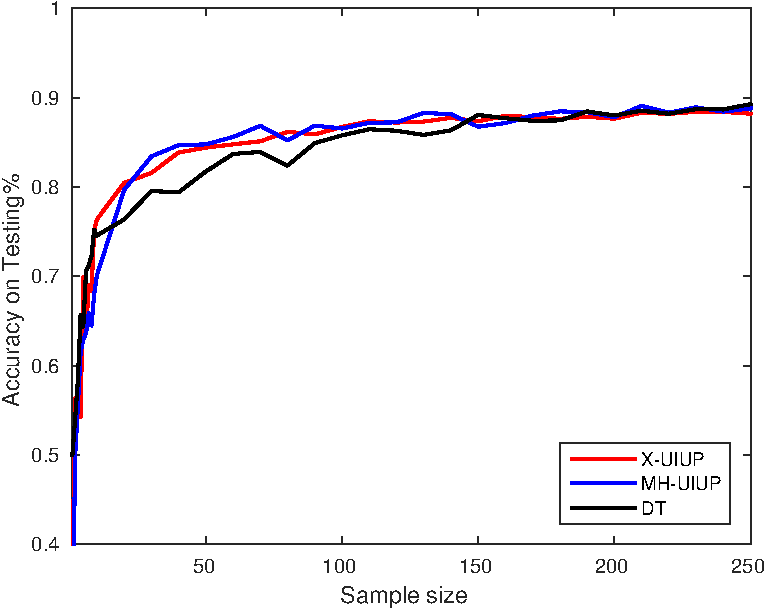
\includegraphics[width=\textwidth]{figs/PLPTF/Trees/BreastCancerWisconsinDownsampled_Trees_X_MH.pdf}
		\caption{BreastCancerWisconsin}
		\label{fig:B1}
	\end{subfigure}
  \begin{subfigure}[b]{0.3\textwidth}
		\centering
  	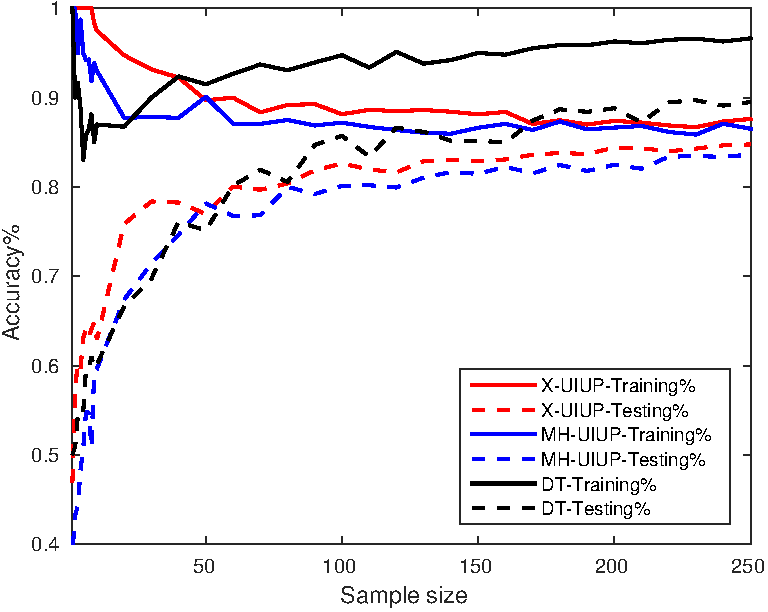
\includegraphics[width=\textwidth]{figs/PLPTF/Trees/CarEvaluation_Trees_X_MH.pdf}
  	\caption{CarEvaluation}
		\label{fig:Car1}
	\end{subfigure}
  \begin{subfigure}[b]{0.3\textwidth}
		\centering
  	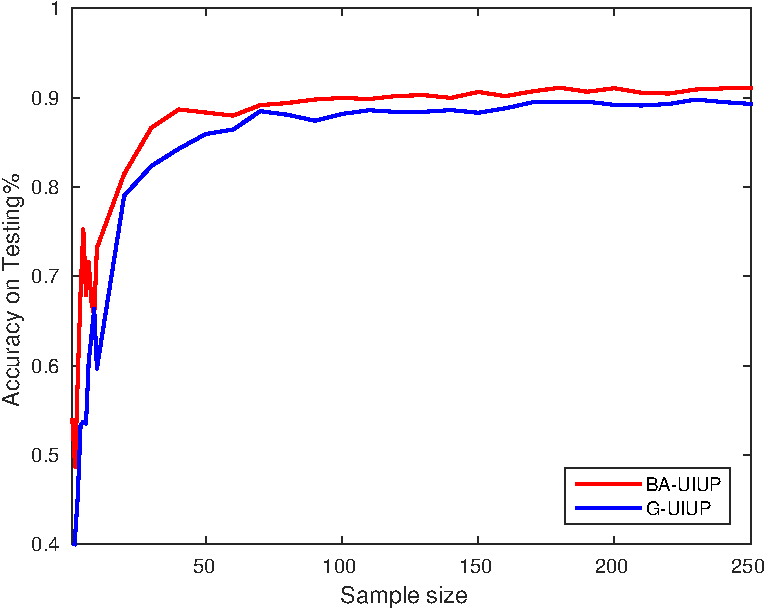
\includegraphics[width=\textwidth]{figs/PLPTF/Trees/CreditApprovalDownsampledFurther_Trees_X_MH.pdf}
  	\caption{CreditApproval}
		\label{fig:Crd1}
	\end{subfigure}
  \\
  \begin{subfigure}[b]{0.3\textwidth}
		\centering
  	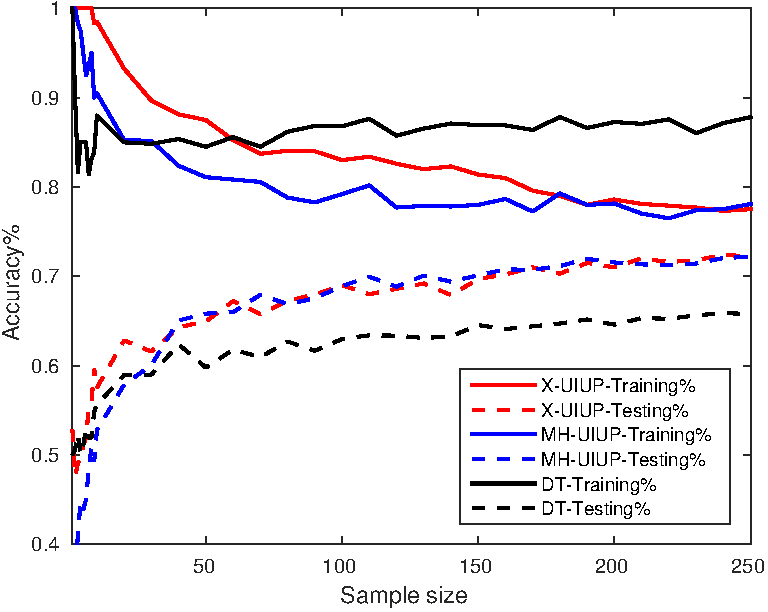
\includegraphics[width=\textwidth]{figs/PLPTF/Trees/GermanCreditDownsampledFurther_Trees_X_MH.pdf}
  	\caption{GermanCredit}
		\label{fig:G1}
	\end{subfigure}
  \begin{subfigure}[b]{0.3\textwidth}
		\centering
  	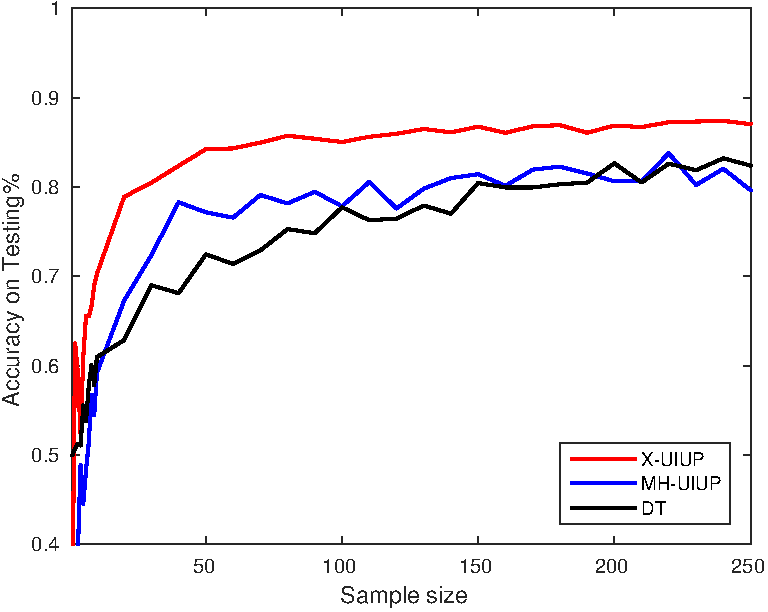
\includegraphics[width=\textwidth]{figs/PLPTF/Trees/IonosphereDownsampledFurther_Trees_X_MH.pdf}
  	\caption{Ionosphere}
		\label{fig:I1}
	\end{subfigure}
  \begin{subfigure}[b]{0.3\textwidth}
		\centering
  	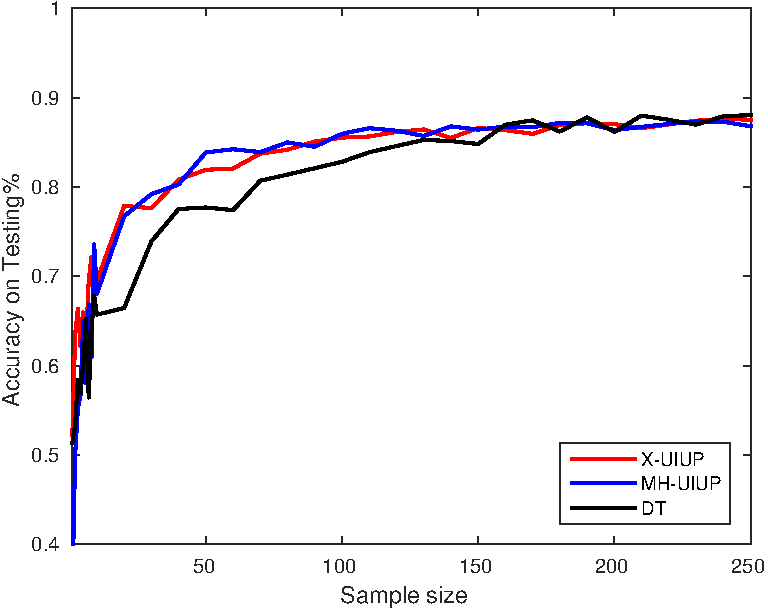
\includegraphics[width=\textwidth]{figs/PLPTF/Trees/MammographicMassDownsampled_Trees_X_MH.pdf}
  	\caption{MammographicMass}
		\label{fig:Mam1}
	\end{subfigure}
	\\
  \begin{subfigure}[b]{0.3\textwidth}
		\centering
  	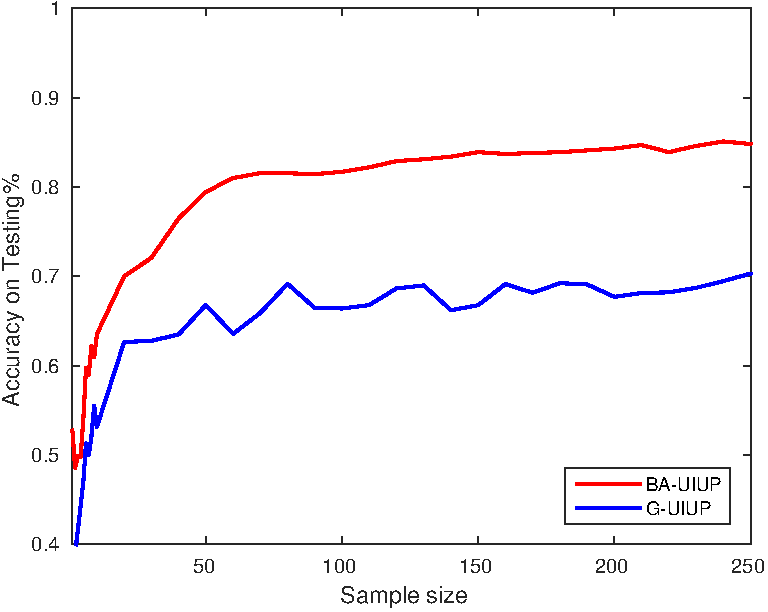
\includegraphics[width=\textwidth]{figs/PLPTF/Trees/MushroomDownsampled_Trees_X_MH.pdf}
  	\caption{Mushroom}
		\label{fig:Mush1}
	\end{subfigure}
  \begin{subfigure}[b]{0.3\textwidth}
		\centering
  	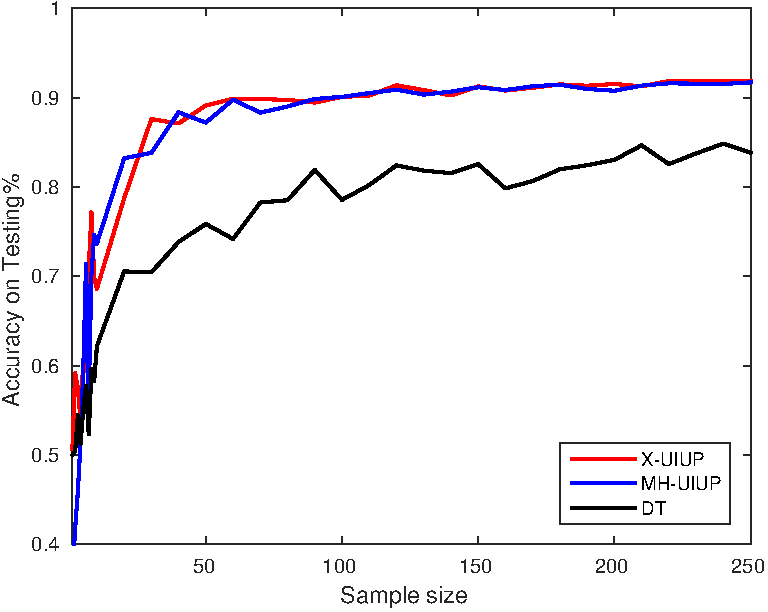
\includegraphics[width=\textwidth]{figs/PLPTF/Trees/NurseryDownsampledFurther_Trees_X_MH.pdf}
  	\caption{Nursery}
		\label{fig:N1}
	\end{subfigure}
  \begin{subfigure}[b]{0.3\textwidth}
		\centering
  	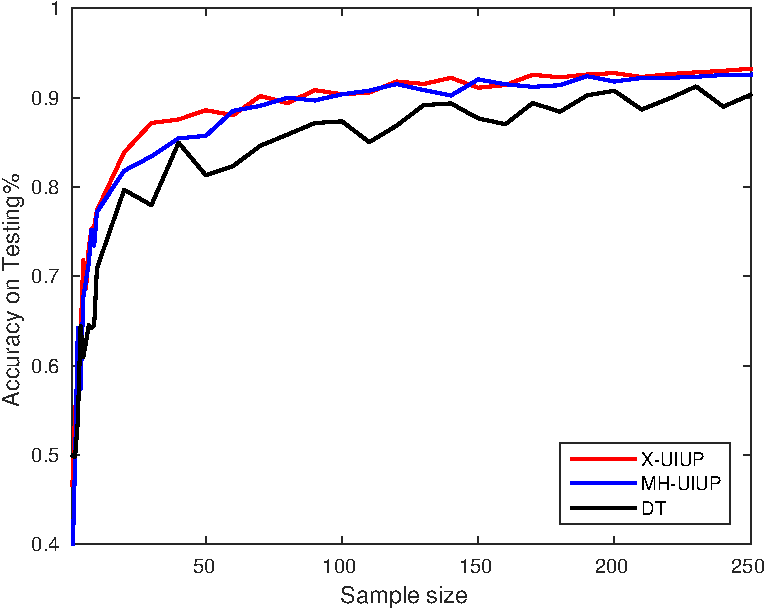
\includegraphics[width=\textwidth]{figs/PLPTF/Trees/SpectHeartDownsampledFurther_Trees_X_MH.pdf}
  	\caption{SpectHeart}
		\label{fig:S1}
	\end{subfigure}
  \\
  \begin{subfigure}[b]{0.3\textwidth}
		\centering
  	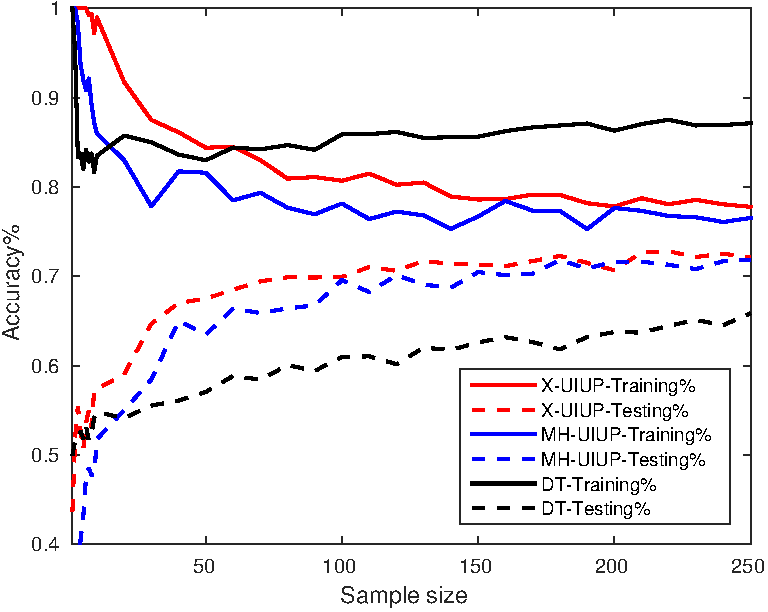
\includegraphics[width=\textwidth]{figs/PLPTF/Trees/TicTacToe_Trees_X_MH.pdf}
  	\caption{TicTacToe}
		\label{fig:T1}
	\end{subfigure}
  \begin{subfigure}[b]{0.3\textwidth}
		\centering
  	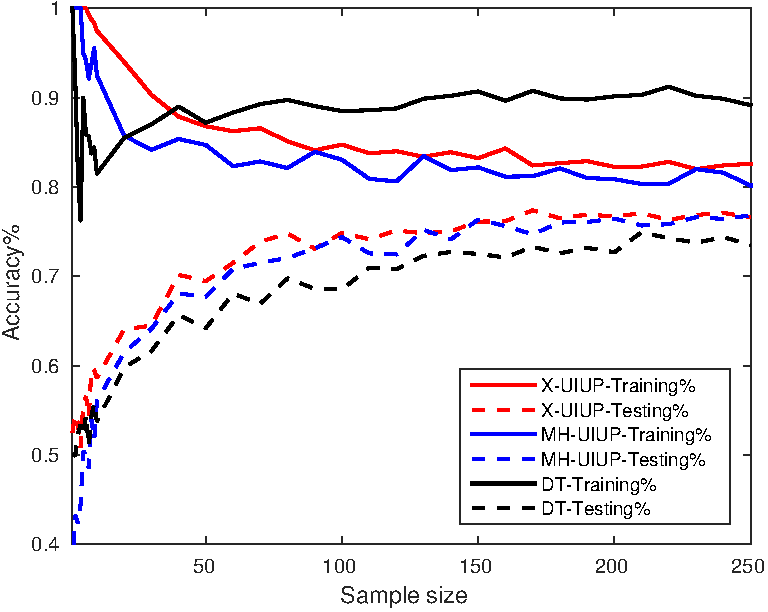
\includegraphics[width=\textwidth]{figs/PLPTF/Trees/VehicleDownsampledFurther_Trees_X_MH.pdf}
  	\caption{Vehicle}
		\label{fig:V1}
	\end{subfigure}
  \begin{subfigure}[b]{0.3\textwidth}
		\centering
  	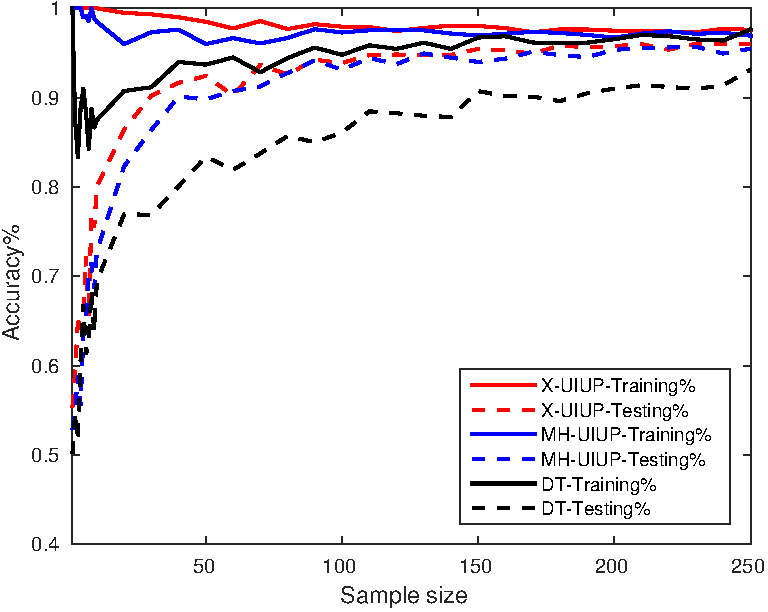
\includegraphics[width=\textwidth]{figs/PLPTF/Trees/WineDownsampled_Trees_X_MH.pdf}
  	\caption{Wine}
		\label{fig:W1}
	\end{subfigure}

  \caption{UIUP PLP-trees vs. decision trees}
  \label{fig:trees1}
\end{figure*}

Next, since X-UIUP does not scale well even for small samples of sizes near
250, we have performed experiments with more expansive samples using the greedy
heuristic on all four classes of PLP-trees: UIUP, UICP-1, CIUP and CICP.
For dataset $\cE^\succ$, we generate $R_{\cE^\succ}$ 
($1\%*|\cE^\succ| \leq |\R_{\cE^\succ}| \leq 70\%*|\cE^\succ|$)
and $\T_{\cE^\succ}$ ($\T_{\cE^\succ}=\cE^\succ \backslash \R_{\cE^\succ}$) 
for training and testing, respectively.
Then, from $\R_{\cE^\succ}$, we train UIUP, UICP-1, CIUP and CICP trees
($T_1$, $T_2$, $T_3$ and $T_4$) using the greedy heuristic.
Finally, on $\T_{\cE^\succ}$ we test the models $T_1$, $T_2$, $T_3$ and $T_4$ to compute the percentages of 
strict examples in $\T_{\cE^\succ}$ that are correctly decided by them.
In \tblref{trees2}, we present results of accuracy on testing using 70\% of $\cE^\succ$
in the training phase.

\begin{table}
  \centering
  \small
  \begin{tabular}{ |c||c|c|c|c| }
    \hline
    Dataset          				& UIUP & UICP-1 & CIUP & CICP \\
    \hline \hline
    BreastCancerWisconsin   & 90.7 & 91.4 & 90.7 & 91.4 \\
    \hline                                            
    CarEvaluation           & 85.8 & 86.0 & 85.9 & 86.0 \\
    \hline                                            
    CreditApproval          & 91.4 & 91.7 & 92.0 & 92.2 \\
    \hline                                            
    GermanCredit            & 74.3 & 74.6 & 74.5 & 75.7 \\
    \hline                                            
    Ionosphere              & 87.1 & [86.9] & 88.5 & 90.4 \\
    \hline                                            
    MammographicMass        & 88.2 & 89.5 & [86.9] & 90.0 \\
    \hline                                            
    Mushroom                & 71.6 & 74.2 & 75.6 & 76.6 \\
    \hline                                            
    Nursery                 & 92.9 & 93.0 & 93.0 & 93.0 \\
    \hline                                            
    SPECTHeart              & 93.4 & 94.9 & 94.8 & 95.7 \\
    \hline                                            
    TicTacToe               & 73.9 & 74.5 & 75.4 & 76.2 \\
    \hline                                            
    Vehicle                 & 79.2 & 80.4 & 80.0 & 81.2 \\
    \hline                                            
    Wine                    & 95.5 & 97.8 & 97.5 & 97.8 \\
    \hline
  \end{tabular}
  \caption{Accuracy percents on the testing data (30\% of $\cE^\succ$)
					 for all four classes of PLP-trees, using models learned
					 by the greedy algorithm from the learning 
					 data (the other 70\% of $\cE^\succ$)}
  \label{tbl:trees2}
\end{table}

What we have learned from \tblref{trees2}:
\begin{enumerate}
	\item UIUP trees performs well, with all datasets above 70\%, and
				4 datasets (GermanCredit,
				Mushroom, TicTacToe and Vehicle) below 85\%.
	\item UICP-1 trees outperforms UIUP trees on all but one dataset
				Ionosphere.
	\item CIUP trees outperforms UIUP trees on all but one dataset
				MammographicMass.
	\item CICP trees outperforms all other classes of trees on all
				datasets.
\end{enumerate}


\subsection{Evaluating PLP-Forests}
To further boost up performances, we now show empirical results
of learning \tit{PLP-forests}.

First, we show results for UIUP PLP-forests using exact learning
and the greedy heuristic.
In each experiment, we randomly partition a dataset into training
set (70\%) and testing set (30\%), learn a forest (the size of it
indicated by on the x-axis) where
each tree is learned from 50 randomly selected examples from the
training set, and test the forest against the testing set.
We repeat it 20 times and report the averge accuracy (indicated on
the y-axis) in the plots.
Note that the plots also include a straight line representing
the result for learning a UIUP PLP-tree, had we used all the
training data to learn a single tree using the greedy heuristic.

\begin{table}
  \centering
  \small
  \begin{tabular}{ |c||c|c|c| }
    \hline
    Dataset          				& MH+Tree & MH+Forest & X+Forest\\
    \hline \hline
    BreastCancerWisconsin   & 90.7 & 93.4 & 95.1 \\
    \hline                                     
    CarEvaluation           & 85.8 & 91.9 & [89.2] \\
    \hline                                     
    CreditApproval          & 91.4 & 91.5 & 93.1 \\
    \hline                                     
    GermanCredit            & 74.3 & 75.4 & 77.9 \\
    \hline                                     
    Ionosphere              & 87.1 & [83.0] & 92.5 \\
    \hline                                     
    MammographicMass        & 88.2 & 89.1 & 90.8 \\
    \hline                                     
    Mushroom                & 71.6 & 78.8 & 90.2 \\
    \hline                                     
    Nursery                 & 92.9 & 93.2 & 94.0 \\
    \hline                                     
    SPECTHeart              & 93.4 & 93.7 & 94.9 \\
    \hline                                     
    TicTacToe               & 73.9 & 75.1 & 77.2 \\
    \hline                                     
    Vehicle                 & 79.2 & 82.7 & [81.9] \\
    \hline                                     
    Wine                    & 95.5 & 95.8 & 96.9 \\
    \hline
  \end{tabular}
  \caption{Accuracy percents on the testing data (30\% of $\cE^\succ$)
					 for UIUP trees and forests of 5000 UIUP trees, 
					 using the greedy and exact algorithms from the learning 
					 data (the other 70\% of $\cE^\succ$)}
  \label{tbl:forests1}
\end{table}

What we have learned from \tblref{forests1}:
\begin{enumerate}
	\item UIUP forests using the greedy method
				outperforms UIUP trees using the greedy method on all
				but one dataset: Ionosphere.
				Average improvement is 1.63\%.
	\item UIUP forests using the exact algorithm
				outperforms UIUP trees using the greedy method on all
				datasets.
				Average improvement is 4.14\%.
	\item UIUP forests using the exact algorithm
				outperforms UIUP forests using the greedy method on all
				but two datasets: CarEvaluation and Vehicle.
				Average improvement is 2.51\%.
\end{enumerate}


Second, we show results for UIUP PLP-forests using the greedy
heuristic with different learning sample size per tree.
The setting is similar to the previous one.
These results are shown in \figref{B4}, \figref{Car4}, \figref{Crd4}, \figref{I4},
\figref{Mam4}, \figref{S4}, \figref{T4}, \figref{V4}, and \figref{W4}.

\begin{figure*}[ht]
	\centering

  \begin{subfigure}[b]{0.3\textwidth}
		\centering
		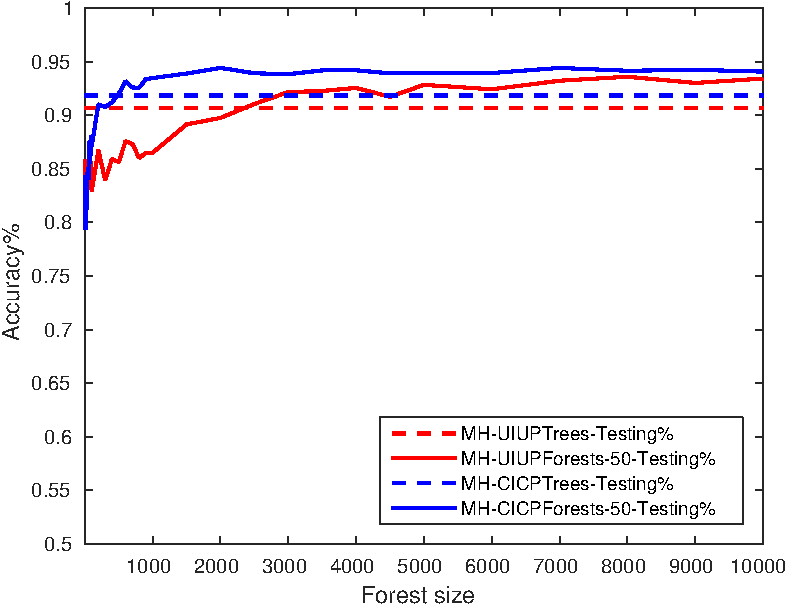
\includegraphics[width=\textwidth]{figs/PLPTF/Forests/BreastCancerWisconsinDownsampled_Forests_MH.pdf}
		\caption{BreastCancerWisconsin}
		\label{fig:B4}
	\end{subfigure}
  \begin{subfigure}[b]{0.3\textwidth}
		\centering
  	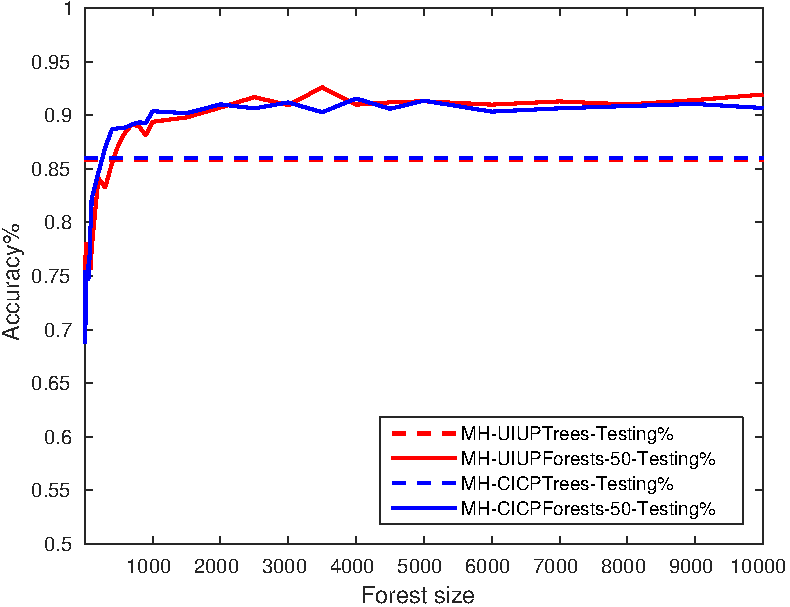
\includegraphics[width=\textwidth]{figs/PLPTF/Forests/CarEvaluation_Forests_MH.pdf}
  	\caption{CarEvaluation}
		\label{fig:Car4}
	\end{subfigure}
  \begin{subfigure}[b]{0.3\textwidth}
		\centering
  	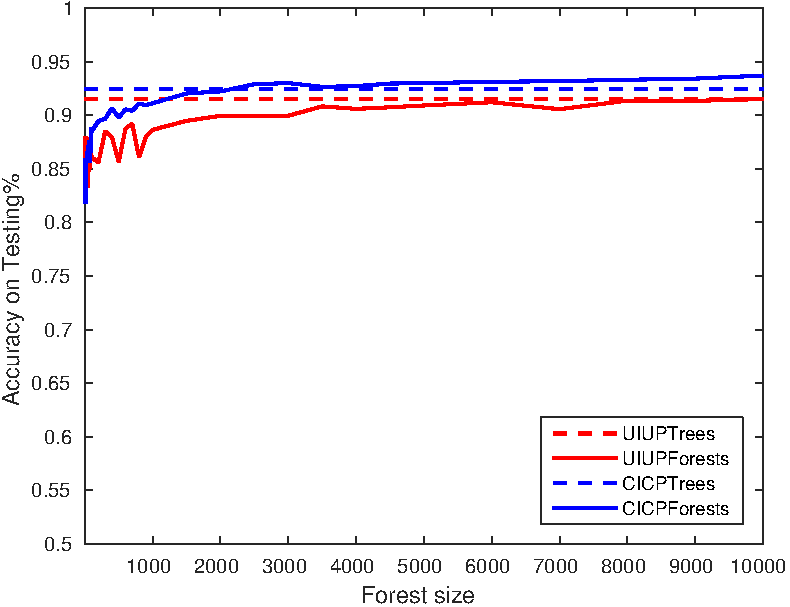
\includegraphics[width=\textwidth]{figs/PLPTF/Forests/CreditApprovalDownsampledFurther_Forests_MH.pdf}
  	\caption{CreditApproval}
		\label{fig:Crd4}
	\end{subfigure}
  \\
  \begin{subfigure}[b]{0.3\textwidth}
		\centering
  	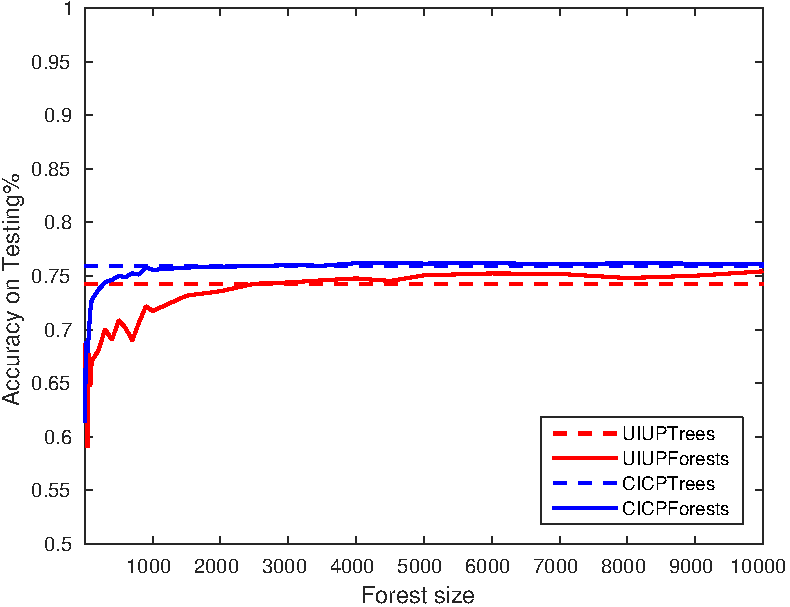
\includegraphics[width=\textwidth]{figs/PLPTF/Forests/GermanCreditDownsampledFurther_Forests_MH.pdf}
  	\caption{GermanCredit}
		\label{fig:G4}
	\end{subfigure}
  \begin{subfigure}[b]{0.3\textwidth}
		\centering
  	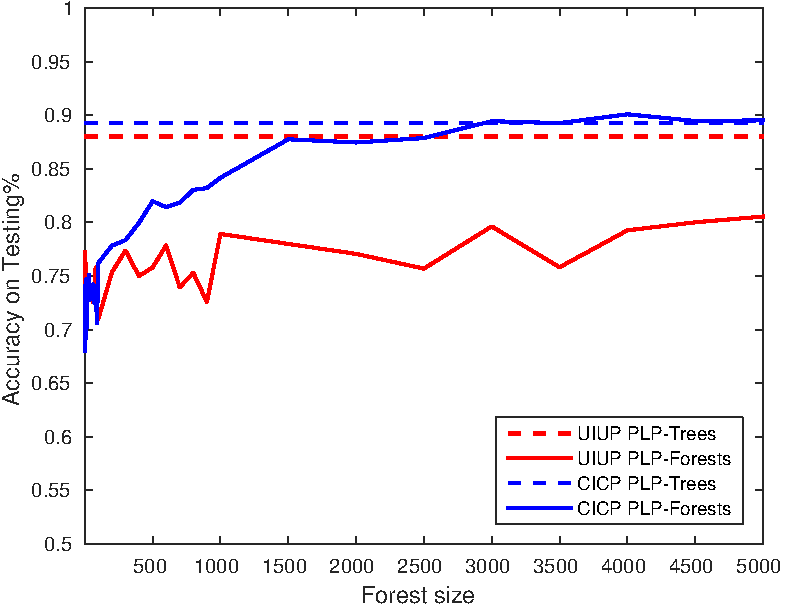
\includegraphics[width=\textwidth]{figs/PLPTF/Forests/IonosphereDownsampledFurther_Forests_MH.pdf}
  	\caption{Ionosphere}
		\label{fig:I4}
	\end{subfigure}
  \begin{subfigure}[b]{0.3\textwidth}
		\centering
  	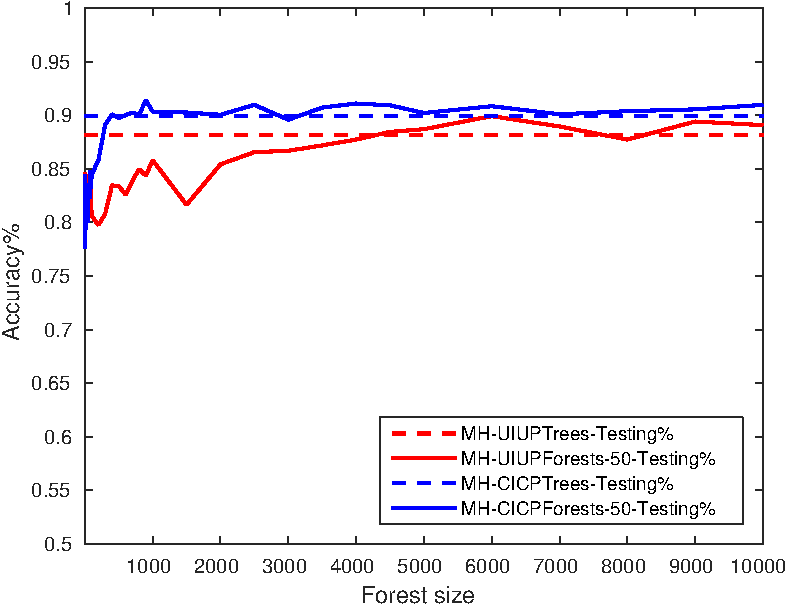
\includegraphics[width=\textwidth]{figs/PLPTF/Forests/MammographicMassDownsampled_Forests_MH.pdf}
  	\caption{MammographicMass}
		\label{fig:Mam4}
	\end{subfigure}
	\\
  \begin{subfigure}[b]{0.3\textwidth}
		\centering
  	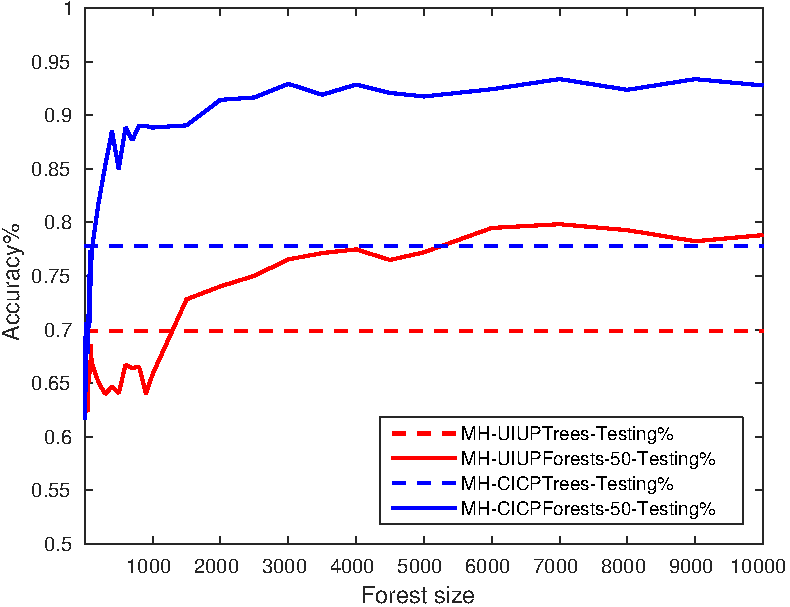
\includegraphics[width=\textwidth]{figs/PLPTF/Forests/MushroomDownsampled_Forests_MH.pdf}
  	\caption{Mushroom}
		\label{fig:Mush4}
	\end{subfigure}
  \begin{subfigure}[b]{0.3\textwidth}
		\centering
  	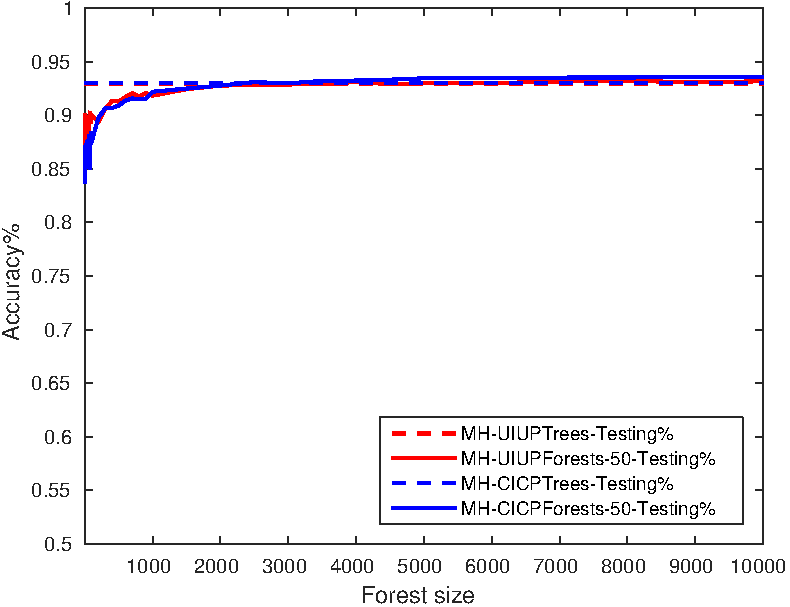
\includegraphics[width=\textwidth]{figs/PLPTF/Forests/NurseryDownsampledFurther_Forests_MH.pdf}
  	\caption{Nursery}
		\label{fig:N4}
	\end{subfigure}
  \begin{subfigure}[b]{0.3\textwidth}
		\centering
  	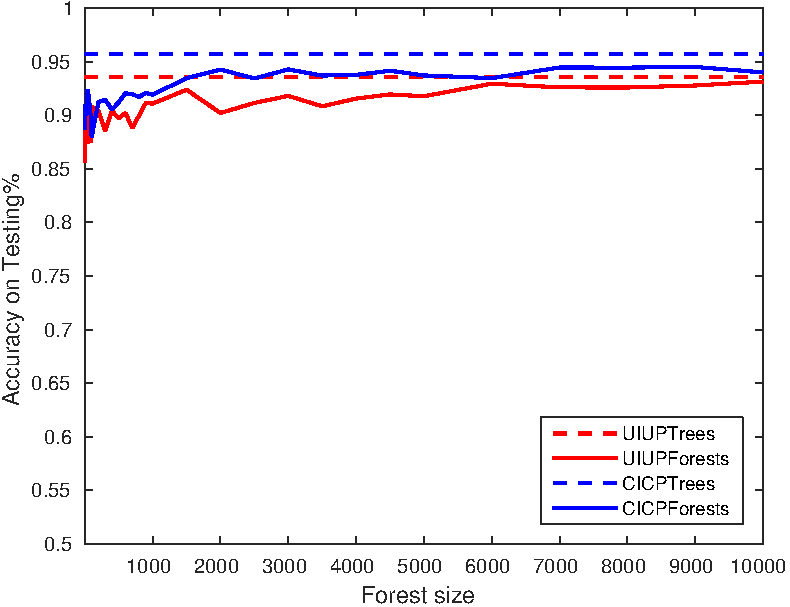
\includegraphics[width=\textwidth]{figs/PLPTF/Forests/SpectHeartDownsampledFurther_Forests_MH.pdf}
  	\caption{SpectHeart}
		\label{fig:S4}
	\end{subfigure}
  \\
  \begin{subfigure}[b]{0.3\textwidth}
		\centering
  	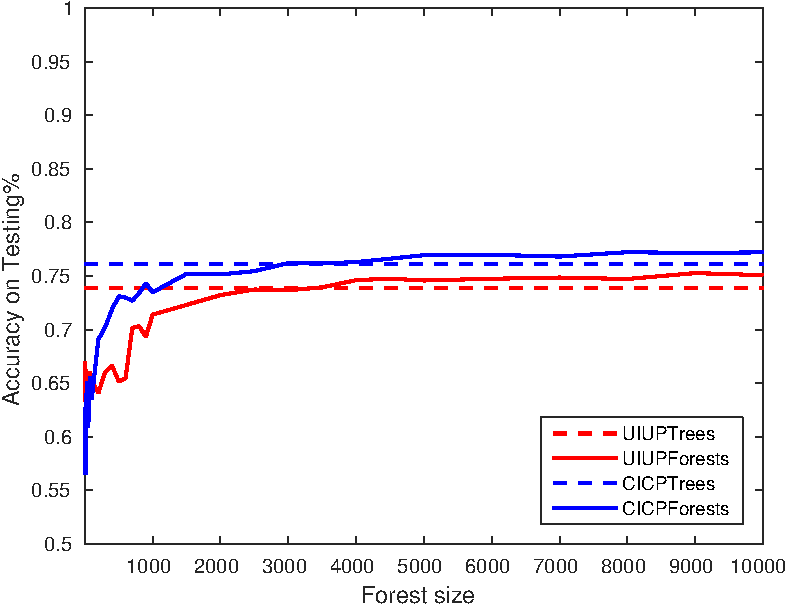
\includegraphics[width=\textwidth]{figs/PLPTF/Forests/TicTacToe_Forests_MH.pdf}
  	\caption{TicTacToe}
		\label{fig:T4}
	\end{subfigure}
  \begin{subfigure}[b]{0.3\textwidth}
		\centering
  	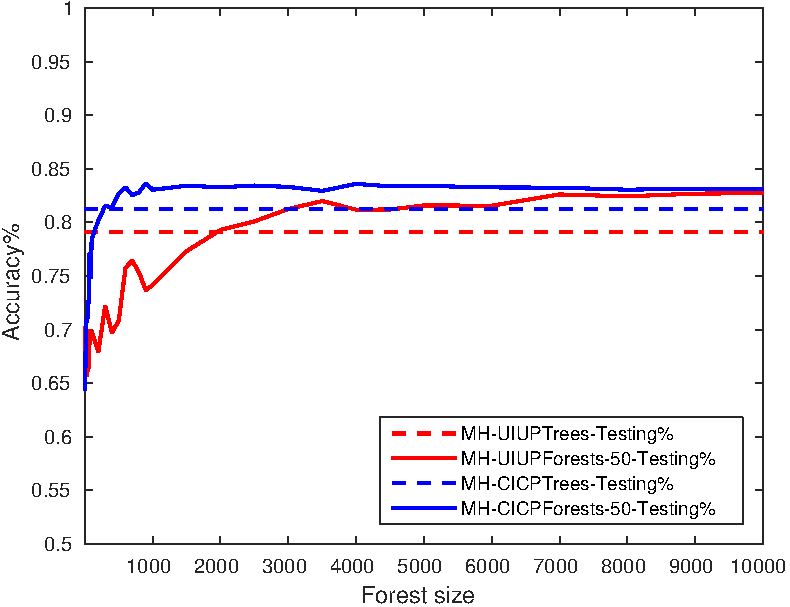
\includegraphics[width=\textwidth]{figs/PLPTF/Forests/VehicleDownsampledFurther_Forests_MH.pdf}
  	\caption{Vehicle}
		\label{fig:V4}
	\end{subfigure}
  \begin{subfigure}[b]{0.3\textwidth}
		\centering
  	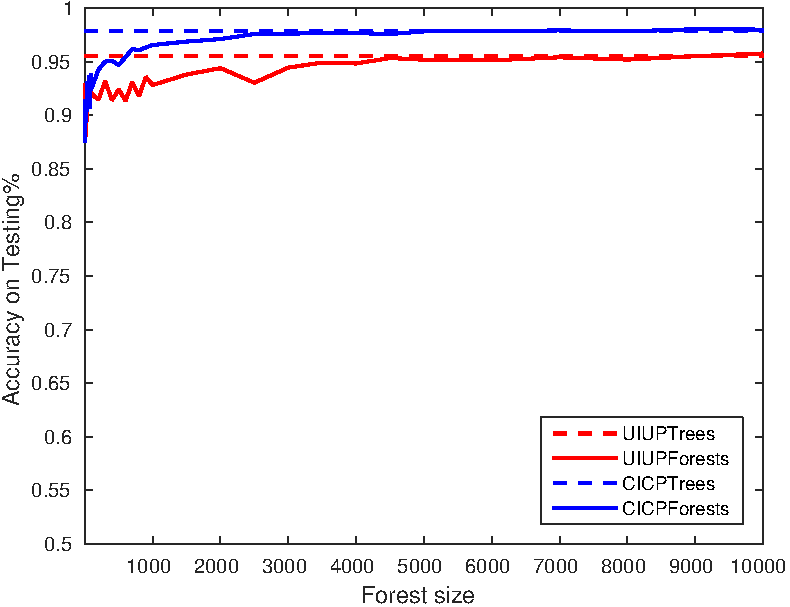
\includegraphics[width=\textwidth]{figs/PLPTF/Forests/WineDownsampled_Forests_MH.pdf}
  	\caption{Wine}
		\label{fig:W4}
	\end{subfigure}

  \caption{Forests of UIUP trees vs. forests of CICP trees}
  \label{fig:forests2}
\end{figure*}

What we have learned from \figref{forests2}:
\begin{enumerate}
	\item CICP forests surpass CICP trees on all but one dataset: SPECTHeart.
	\item UIUP forests surpass CICP trees on 4 datasets, and fall short on the others.
	\item CICP forests dominate UIUP forests on 10 datasets, and perform very close on
				the other 2.
\end{enumerate}


\section{Conclusion and Future Work}
In this paper, we reviewed different classifications of PLP-trees,
and introduced \tit{partial lexicographic preference forests},
or \tit{PLP-forests}, to reduce the high variance of PLP-trees.
To support experimentation, we have constructed a preference
learning library from existing reservoir of classification
datasets.
To this end, we implemented an \tit{exact} learner using
\tit{answer-set programming}, and an \tit{approximation}
learner using a straightforward greedy heuristic.
Our empirical results on PLP-trees show that the language offers
high accuracy, mostly higher than decision trees when training samples
are small.
For PLP-forests, we have observed improvements, significant in some cases,
from single tree models.

Looking into the future, we are interested in expanding our preference
learning library by creating real-work datasets through
conducting experiments involving human subjects.
We also plan to implement and experiment with other aggregators
for PLP-forests, and compare with our results using
the desirable and intuitive majority rule.
